% Options for packages loaded elsewhere
\PassOptionsToPackage{unicode}{hyperref}
\PassOptionsToPackage{hyphens}{url}
%
\documentclass[
]{book}
\title{설치형 오픈 통계 패키지 - \texttt{Rcmdr}}
\author{신종화, 이광춘, 유충현, 홍성학}
\date{2022-04-16}

\usepackage{amsmath,amssymb}
\usepackage{lmodern}
\usepackage{iftex}
\ifPDFTeX
  \usepackage[T1]{fontenc}
  \usepackage[utf8]{inputenc}
  \usepackage{textcomp} % provide euro and other symbols
\else % if luatex or xetex
  \usepackage{unicode-math}
  \defaultfontfeatures{Scale=MatchLowercase}
  \defaultfontfeatures[\rmfamily]{Ligatures=TeX,Scale=1}
\fi
% Use upquote if available, for straight quotes in verbatim environments
\IfFileExists{upquote.sty}{\usepackage{upquote}}{}
\IfFileExists{microtype.sty}{% use microtype if available
  \usepackage[]{microtype}
  \UseMicrotypeSet[protrusion]{basicmath} % disable protrusion for tt fonts
}{}
\makeatletter
\@ifundefined{KOMAClassName}{% if non-KOMA class
  \IfFileExists{parskip.sty}{%
    \usepackage{parskip}
  }{% else
    \setlength{\parindent}{0pt}
    \setlength{\parskip}{6pt plus 2pt minus 1pt}}
}{% if KOMA class
  \KOMAoptions{parskip=half}}
\makeatother
\usepackage{xcolor}
\IfFileExists{xurl.sty}{\usepackage{xurl}}{} % add URL line breaks if available
\IfFileExists{bookmark.sty}{\usepackage{bookmark}}{\usepackage{hyperref}}
\hypersetup{
  pdftitle={설치형 오픈 통계 패키지 - Rcmdr},
  pdfauthor={신종화, 이광춘, 유충현, 홍성학},
  hidelinks,
  pdfcreator={LaTeX via pandoc}}
\urlstyle{same} % disable monospaced font for URLs
\usepackage{color}
\usepackage{fancyvrb}
\newcommand{\VerbBar}{|}
\newcommand{\VERB}{\Verb[commandchars=\\\{\}]}
\DefineVerbatimEnvironment{Highlighting}{Verbatim}{commandchars=\\\{\}}
% Add ',fontsize=\small' for more characters per line
\usepackage{framed}
\definecolor{shadecolor}{RGB}{248,248,248}
\newenvironment{Shaded}{\begin{snugshade}}{\end{snugshade}}
\newcommand{\AlertTok}[1]{\textcolor[rgb]{0.94,0.16,0.16}{#1}}
\newcommand{\AnnotationTok}[1]{\textcolor[rgb]{0.56,0.35,0.01}{\textbf{\textit{#1}}}}
\newcommand{\AttributeTok}[1]{\textcolor[rgb]{0.77,0.63,0.00}{#1}}
\newcommand{\BaseNTok}[1]{\textcolor[rgb]{0.00,0.00,0.81}{#1}}
\newcommand{\BuiltInTok}[1]{#1}
\newcommand{\CharTok}[1]{\textcolor[rgb]{0.31,0.60,0.02}{#1}}
\newcommand{\CommentTok}[1]{\textcolor[rgb]{0.56,0.35,0.01}{\textit{#1}}}
\newcommand{\CommentVarTok}[1]{\textcolor[rgb]{0.56,0.35,0.01}{\textbf{\textit{#1}}}}
\newcommand{\ConstantTok}[1]{\textcolor[rgb]{0.00,0.00,0.00}{#1}}
\newcommand{\ControlFlowTok}[1]{\textcolor[rgb]{0.13,0.29,0.53}{\textbf{#1}}}
\newcommand{\DataTypeTok}[1]{\textcolor[rgb]{0.13,0.29,0.53}{#1}}
\newcommand{\DecValTok}[1]{\textcolor[rgb]{0.00,0.00,0.81}{#1}}
\newcommand{\DocumentationTok}[1]{\textcolor[rgb]{0.56,0.35,0.01}{\textbf{\textit{#1}}}}
\newcommand{\ErrorTok}[1]{\textcolor[rgb]{0.64,0.00,0.00}{\textbf{#1}}}
\newcommand{\ExtensionTok}[1]{#1}
\newcommand{\FloatTok}[1]{\textcolor[rgb]{0.00,0.00,0.81}{#1}}
\newcommand{\FunctionTok}[1]{\textcolor[rgb]{0.00,0.00,0.00}{#1}}
\newcommand{\ImportTok}[1]{#1}
\newcommand{\InformationTok}[1]{\textcolor[rgb]{0.56,0.35,0.01}{\textbf{\textit{#1}}}}
\newcommand{\KeywordTok}[1]{\textcolor[rgb]{0.13,0.29,0.53}{\textbf{#1}}}
\newcommand{\NormalTok}[1]{#1}
\newcommand{\OperatorTok}[1]{\textcolor[rgb]{0.81,0.36,0.00}{\textbf{#1}}}
\newcommand{\OtherTok}[1]{\textcolor[rgb]{0.56,0.35,0.01}{#1}}
\newcommand{\PreprocessorTok}[1]{\textcolor[rgb]{0.56,0.35,0.01}{\textit{#1}}}
\newcommand{\RegionMarkerTok}[1]{#1}
\newcommand{\SpecialCharTok}[1]{\textcolor[rgb]{0.00,0.00,0.00}{#1}}
\newcommand{\SpecialStringTok}[1]{\textcolor[rgb]{0.31,0.60,0.02}{#1}}
\newcommand{\StringTok}[1]{\textcolor[rgb]{0.31,0.60,0.02}{#1}}
\newcommand{\VariableTok}[1]{\textcolor[rgb]{0.00,0.00,0.00}{#1}}
\newcommand{\VerbatimStringTok}[1]{\textcolor[rgb]{0.31,0.60,0.02}{#1}}
\newcommand{\WarningTok}[1]{\textcolor[rgb]{0.56,0.35,0.01}{\textbf{\textit{#1}}}}
\usepackage{longtable,booktabs,array}
\usepackage{calc} % for calculating minipage widths
% Correct order of tables after \paragraph or \subparagraph
\usepackage{etoolbox}
\makeatletter
\patchcmd\longtable{\par}{\if@noskipsec\mbox{}\fi\par}{}{}
\makeatother
% Allow footnotes in longtable head/foot
\IfFileExists{footnotehyper.sty}{\usepackage{footnotehyper}}{\usepackage{footnote}}
\makesavenoteenv{longtable}
\usepackage{graphicx}
\makeatletter
\def\maxwidth{\ifdim\Gin@nat@width>\linewidth\linewidth\else\Gin@nat@width\fi}
\def\maxheight{\ifdim\Gin@nat@height>\textheight\textheight\else\Gin@nat@height\fi}
\makeatother
% Scale images if necessary, so that they will not overflow the page
% margins by default, and it is still possible to overwrite the defaults
% using explicit options in \includegraphics[width, height, ...]{}
\setkeys{Gin}{width=\maxwidth,height=\maxheight,keepaspectratio}
% Set default figure placement to htbp
\makeatletter
\def\fps@figure{htbp}
\makeatother
\setlength{\emergencystretch}{3em} % prevent overfull lines
\providecommand{\tightlist}{%
  \setlength{\itemsep}{0pt}\setlength{\parskip}{0pt}}
\setcounter{secnumdepth}{5}
\usepackage{booktabs}
\usepackage{amsthm}
\makeatletter
\def\thm@space@setup{%
  \thm@preskip=8pt plus 2pt minus 4pt
  \thm@postskip=\thm@preskip
}
\makeatother
\ifLuaTeX
  \usepackage{selnolig}  % disable illegal ligatures
\fi
\usepackage[]{natbib}
\bibliographystyle{apalike}

\begin{document}
\maketitle

{
\setcounter{tocdepth}{1}
\tableofcontents
}
\hypertarget{uxb4e4uxc5b4uxac00uxba70}{%
\chapter{들어가며}\label{uxb4e4uxc5b4uxac00uxba70}}

\textbf{한국 알(R) 사용자회}는 디지털 불평등 해소와 통계 대중화를 오픈 통계 패키지 개발을 2021년부터 추진하였습니다.
더불어 설치형 오픈 통계 패키지를 신종화 님께서 John Fox 교수님이 개발한 \texttt{Rcmdr} 기반으로 한글화 및 문서화에 10년 넘게 기여해주셨습니다. 이에 \textbf{한국 알(R) 사용자회}는 신종화님의 \texttt{Rcmdr} 거인의 어깨위에 디지털 불평등 해소와 통계 대중화를 위해 한 걸음 더 나아가게 되었습니다. 특히 신종화님께서 기여하신 한글화 및 문서를 근간으로 더 많은 분들이 오픈 통계 패키지를 사용할 수 있도록 \texttt{bookdown}으로 내용을 정리하여 통계 대중화가 한층 앞당겨질 것으로 기대됩니다.

신종화님께서 왜 오픈 통계 패키지로 \texttt{Rcmdr}를 근간으로 해야 하는지 이유를 명쾌하게 다음과 같이 정리해 주셨습니다.

R에는 여러 개의 GUI 작업도구들이 있습니다. 모두 목적이 분명하고, 좋은 도구이며, 일부는 현재도 향상작업이 진행되고 있습니다. 그럼에도 불구하고 R Commander를 위한 블로그 작업을 진행하는 이유는 크게 두가지 입니다.

첫째, R Commander는 직관적으로 기존의 기초통계학 도구와 유사합니다. Command Line 에서 작업하는 것에 익숙하지 않은, 또 어려움을 겪고 있는 사용자들에게 기초통계학분야를 학습하고 활용하는데 도움을 주기 위하여 R Commander가 개발되었습니다. 개발자인 John Fox 교수는 이 목적과 관리방향을 분명히하고 있습니다. 중급이상의 R 사용자/ 고급통계 연구자들에게는 R Commander가 불필요할 수 있습니다.

둘째, 지난 10년동안 R Commander의 메뉴 한글화작업을 진행해왔으며, 현재도 유지관리를 하고 있습니다. (이 정보는 R Commander 안의 Help \textgreater{} About Rcmdr 에 있습니다) {[}Translations: Korean, Chel Hee Lee, Dae-Heung Jang, and Shin Jong-Hwa{]} 지난 10년 동안 개인적인 메모 차원에서 R Commander 사용 및 한글화 관련 블로그 포스트를 만들고 관리되어 왔고 \href{http://modernity.tistory.com}{블로그}에 전체 과정이 고스란히 남아있고 계속적으로 유지관리될 것입니다.

\begin{itemize}
\tightlist
\item
  신종화 \href{https://rcmdr.kr/}{Rcmdr : R Commander}
\item
  \href{https://cran.r-project.org/web/packages/Rcmdr/index.html}{CRAN Rcmdr 패키지 정보}
\item
  \href{https://socialsciences.mcmaster.ca/jfox/Misc/Rcmdr/}{개발자 John Fox 교수의 Rcmdr 소개}
\item
  \href{https://modernity.tistory.com/}{FOSSER\_Ricoop}
\end{itemize}

\hypertarget{install}{%
\chapter{설치}\label{install}}

\hypertarget{uxb3c4uxc6c0uxb9d0-help}{%
\chapter{\texorpdfstring{도움말 / \texttt{Help}}{도움말 / Help}}\label{uxb3c4uxc6c0uxb9d0-help}}

\hypertarget{commander-help-0}{%
\section{Commander help (0)}\label{commander-help-0}}

\hypertarget{introduction-to-the-r-comma..-0}{%
\section{Introduction to the R Comma.. (0)}\label{introduction-to-the-r-comma..-0}}

\hypertarget{r-commander-website-0}{%
\section{R Commander website (0)}\label{r-commander-website-0}}

\hypertarget{about-rcmdr-0}{%
\section{About Rcmdr (0)}\label{about-rcmdr-0}}

\hypertarget{r-commander-hex-sticker}{%
\section{R Commander hex sticker}\label{r-commander-hex-sticker}}

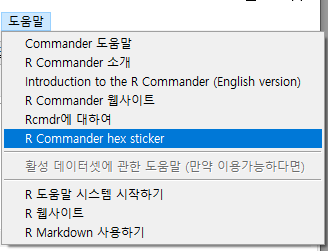
\includegraphics{fig/help-01.png}

선택하면 아래와 같은 이미지 파일이 등장한다:


\includegraphics{fig/help-02.png}

\hypertarget{help-on-active-data-set-if..-0}{%
\section{Help on active data set (if.. (0)}\label{help-on-active-data-set-if..-0}}

\hypertarget{start-r-help-system-0}{%
\section{Start R help system (0)}\label{start-r-help-system-0}}

\hypertarget{r-website-0}{%
\section{R website (0)}\label{r-website-0}}

\hypertarget{using-r-markdown-0}{%
\section{Using R Markdown (0)}\label{using-r-markdown-0}}

\hypertarget{uxb370uxc774uxd130uxc14b-datasets}{%
\chapter{\texorpdfstring{데이터셋 / \texttt{datasets}}{데이터셋 / datasets}}\label{uxb370uxc774uxd130uxc14b-datasets}}

\hypertarget{prestige---cardata-prestige}{%
\section{\texorpdfstring{Prestige - \texttt{carData\ \textgreater{}\ Prestige}}{Prestige - carData \textgreater{} Prestige}}\label{prestige---cardata-prestige}}

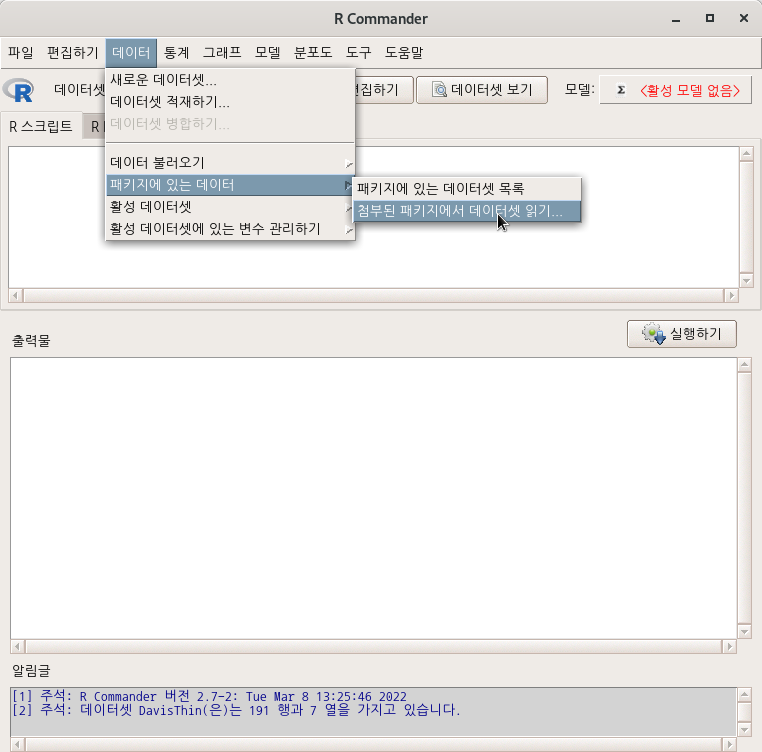
\includegraphics{fig/dataset-prestiage-01.png}

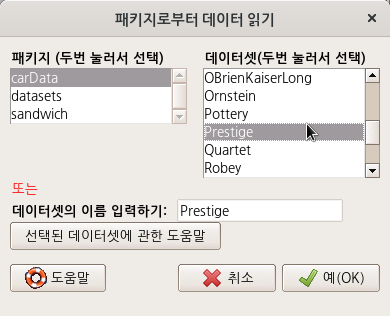
\includegraphics{fig/dataset-prestiage-02.png}

\begin{Shaded}
\begin{Highlighting}[]
\FunctionTok{data}\NormalTok{(Prestige, }\AttributeTok{package=}\StringTok{"carData"}\NormalTok{)}
\end{Highlighting}
\end{Shaded}

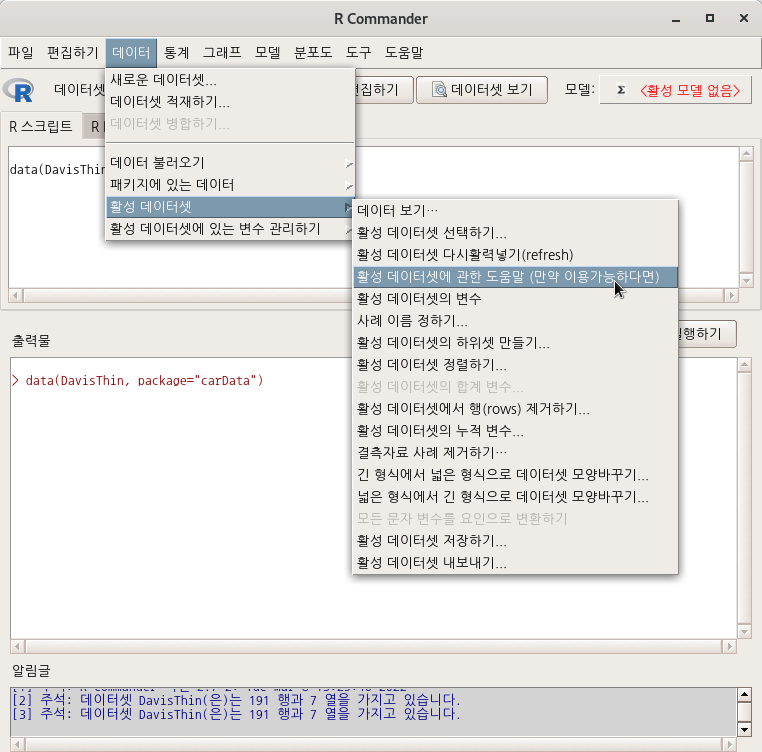
\includegraphics{fig/dataset-prestiage-03.png}

\begin{Shaded}
\begin{Highlighting}[]
\FunctionTok{help}\NormalTok{(}\StringTok{"Prestige"}\NormalTok{)}
\end{Highlighting}
\end{Shaded}

carData 패키지에 있는 Prestige 데이터셋을 \texttt{.csv}로 저장하여 내보낼 수 있다.

\href{data/Prestige.csv}{다운로드}

참조: \href{https://rcmdr.tistory.com/52}{활성 데이터셋 내보내기\ldots{}}

\hypertarget{moore---cardata-moore}{%
\section{\texorpdfstring{Moore - \texttt{carData\ \textgreater{}\ Moore}}{Moore - carData \textgreater{} Moore}}\label{moore---cardata-moore}}

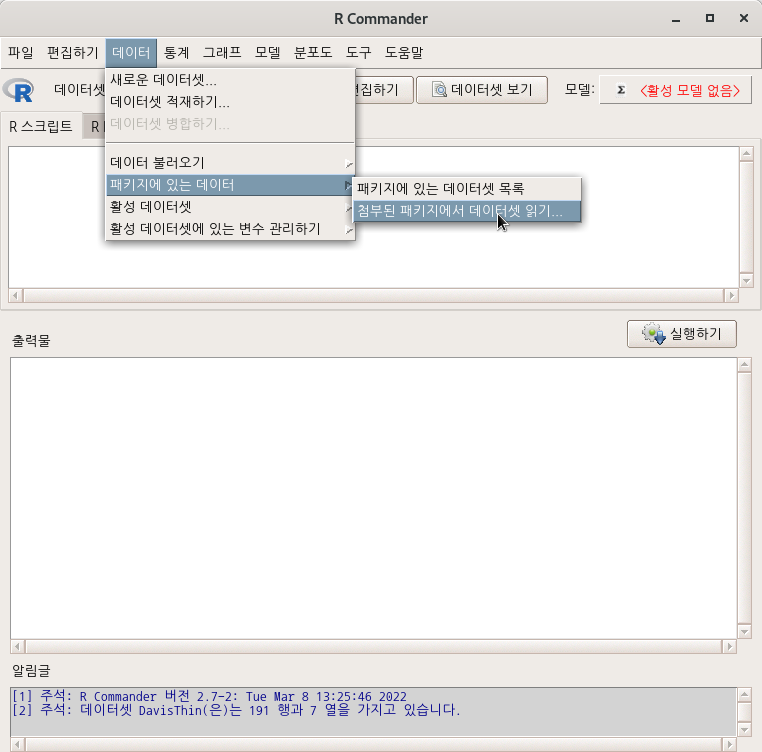
\includegraphics{fig/dataset-moore-01.png}

Moore \{carData\}

R Documentation

Status, Authoritarianism, and Conformity

Description

The Moore data frame has 45 rows and 4 columns.
The data are for subjects in a social-psychological experiment,
who were faced with manipulated disagreement from a partner of either
of low or high status. The subjects could either conform to the
partner's judgment or stick with their own judgment.

Usage

Format

This data frame contains the following columns:

partner.status

Partner's status. A factor with levels:
high,
low.

conformity

Number of conforming responses in 40 critical trials.

fcategory

F-Scale Categorized.
A factor with levels (note levels out of order):
high,
low,
medium.

fscore

Authoritarianism: F-Scale score.

Source

Moore, J. C., Jr.~and Krupat, E. (1971)
Relationship between source status, authoritarianism and conformity in a
social setting. Sociometry 34, 122--134.

Personal communication
from J. Moore, Department of Sociology, York University.

References

Fox, J. (2016)
Applied Regression Analysis and Generalized Linear Models,
Third Edition. Sage.

Fox, J. and Weisberg, S. (2019)
An R Companion to Applied Regression, Third Edition, Sage.

{[}Package carData version 3.0-5 Index{]}

\hypertarget{obrienkaiser-2}{%
\section{OBrienKaiser (2)}\label{obrienkaiser-2}}

\hypertarget{obrienkaiserlong-1}{%
\section{OBrienKaiserLong (1)}\label{obrienkaiserlong-1}}

\hypertarget{airquality-2}{%
\section{airquality (2)}\label{airquality-2}}

\hypertarget{bfox-1}{%
\section{Bfox (1)}\label{bfox-1}}

\hypertarget{sleep-1}{%
\section{sleep (1)}\label{sleep-1}}

\hypertarget{davisthin-1}{%
\section{DavisThin (1)}\label{davisthin-1}}

\hypertarget{usarrests-1}{%
\section{USArrests (1)}\label{usarrests-1}}

\hypertarget{birthwt-1}{%
\section{birthwt (1)}\label{birthwt-1}}

\hypertarget{friendly-1}{%
\section{Friendly (1)}\label{friendly-1}}

\hypertarget{cowles-1}{%
\section{Cowles (1)}\label{cowles-1}}

\hypertarget{adler-1}{%
\section{Adler (1)}\label{adler-1}}

\hypertarget{warpbreaks-1}{%
\section{warpbreaks (1)}\label{warpbreaks-1}}

  \bibliography{book.bib,packages.bib}

\end{document}
